\chapter{Optimal experiment design}
\label{sec:OptimalExperimentDesign}

In the diabetes research scenario, the fact of performing experiments is a high-cost, time consuming task that has to be thoroughly planned in order to obtain the biggest benefit out of it. In the case that is being reviewed in here, the objective of that planning is to get the models to be easier to identify. There are some methods that will help the researcher to obtain the best identifiability of a given model, choosing from a constrained set of possible experiments.

An experiment of data recollection in diabetes initially has infinite number of variables that can change under different circumstances. The models chosen is the first choice to be made, and it is not an obvious one. In this thesis case the models have already been chosen, but for the optimal experiment design only the two minimal models will be used. The reason of that decision is simply of computational effort. The experiment design implies solving optimization problems whose computation times depends on the complexity of the models, and those times are usually very long.

The design of an optimal experiment usually consists of the following steps:
\begin{enumerate}
	\item Define an optimality criterion related to the final purpose of the modeling, in this case optimal identifiability, \textit{via} a scalar cost function.
	\item Take into account all constraints on feasible experiments.
	\item Optimize the chosen cost function with respect to the experimental variables available to the experimenter.
\end{enumerate}
The experiment design will usually result in a non-linear constrained optimization problem and thus, global optimization solvers will be needed in order to find the solution. In this chapter there will be a justification of the optimal experiment design in diabetes, followed by the formulation necessary to define the criterion of optimality for identification. Finally results of optimal designs will be shown.

\section{The need of optimal design}
\label{sec:TheNeedOfOptimalDesign}

There is a classical example seen in \cite{walter1997} that explains very clearly the need of optimal design for almost every experiment to be performed. That example will be reproduced in the following lines, showing that usually the intuitive approach for experimentation is not optimal.

\subsubsection{Example.-}
\label{sec:Example}

\textit{There are three objects called $O_{1}$, $O_{2}$ and $O_{3}$ with respective weights $w_{1}^{*}$, $w_{2}^{*}$ and $w_{3}^{*}$ to be estimated. The spring balance used for this purpose produces a biased random measurement error, defined by a Gaussian distribution $\mathcal{N}(0,\sigma^{2})$ and the measurement bias $w_{0}^{*}$. Only four measurements can be done in this experiment.}

\textit{Intuition dictates to do the first of the measurements $y(0)$ without any object on the balance, in order to characterize the bias, and then have the other three resting measurements for each of the objects. In that case the estimates of the weight for each object is $\hat{w}_{i}=y(i)-y(0),\ i=1,\ 2,\ 3$. The estimates in this case are unbiased (which is very good), and have variances $var(\hat{w}_{i})=2\sigma^{2}$ and covariances $cov(\hat{w}_{i},\hat{w}_{j})=\sigma^{2},\ i\neq j$.}

\textit{Another case has to be considered now. If the first measurement is now taken with all the objects in the balance, being then $y(0)=w_{0}^{*}+w_{1}^{*}+w_{2}^{*}+w_{3}^{*}$, the estimates of the weights for the objects are:}
\begin{equation}
	\hat{w}_{i}=\frac{y(0)+y(i)-y(j)-y(k)}{2},\ i=1,\ 2,\ 3,\ i\neq j,\ i\neq k,\ j\neq k
\label{eq:example1}
\end{equation}
\textit{In this case, the variances of the estimators, which is a good approximation of the identification performance, are $var(\hat{w}_{i})=\sigma^{2}$ and its covariances $cov(\hat{w}_{i},\hat{w}_{j})=0,\ i\neq j$. Compared to the first intuitive approach, this second approach yields to a more accurate estimation and independent estimates, plus the estimation is also unbiased.}

In the context of the artificial pancreas there are few published examples of experiment design, and even fewer of them are based on the optimality of the experiment in terms of identifiability. One of the earliest attempt to improve the identification in an endogenous model was carried out Cobelli in 1986 \cite{cobelli1987minimal}. The approach is based in the FIM methodology that will be explained in Section \ref{sec:MethodsBasedOnTheFIM}, and it is the same method that will be used in the work done in this thesis. Cobelli though, used a simplified version of experimental design evaluating only the identifiability of single parameters instead of evaluating the identifiability of the model as a block, combining the identifiability of different parameters.

There are several examples of modified standard protocols to perform better identifications, like the work of Percival et al. \cite{percival} where it is proven that simply by separating the instants of insulin bolus injection and the beginning of the meal the identification of a model is improved. However, no theoretical study is presented with this regard.

Only in the last years publications have appeared with complete identifiability studies and optimal design for the identification in diabetes. Galvanin \cite{galvanin2009} published a study of optimal experiments based on Hovorka's model, checking identifiability involving meal ingestion or oral glucose intake, yielding in quite complex insulin infusion rates like the one shown in Figure \ref{fig:insulingalvanin}.

\begin{figure}[hbtp]
\centering
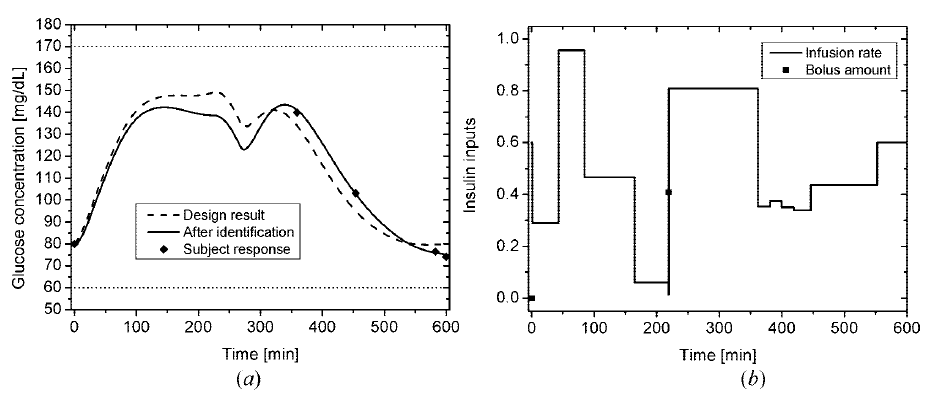
\epsfig{file=Figures/insulingalvanin.png, width=\textwidth}\caption{(a) Glucose concentration profiles predicted by Hovorka's model (dashed line) and after identification (solid line). (b) Insulin infusion rate designed for the identification. Extracted from \cite{galvanin2009}}
\label{fig:insulingalvanin}
\end{figure}

Given the huge problem that identification of models supposes in the artificial pancreas environment, it seems logical to ease the problem as much as possible. In this thesis work several approaches to optimal experiment design based on different models using the FIM methods will be carried out as stated in Section \ref{sec:OptimalDesignResults}.

\section{Methods based on the FIM}
\label{sec:MethodsBasedOnTheFIM}

The aim and need of the experiment design is now clear, and the question of how to perform that design arises. So far, identifiability has been analyzed as a property of a parameter, quantified as the confidence interval in the estimation of each parameter. That information is obtained from the Fisher Information Matrix (or better said from its inverse), which summarizes the information of all the parameters of the model for a given experiment. The problem of optimal design can be expressed then as an optimization problem of finding the minimum value of a certain scalar function of the FIM. That function is called optimality criteria, and its general expression is:
\begin{equation}
	j(\mathbf{\Xi})=\phi[F(\mathbf{p}, \mathbf{\Xi})] \\
\label{eq:index}
\end{equation}
where $\phi$ is a scalar function. The evaluation of the Fisher Information Matrix is a function $F$ of $\mathbf{p}$, the parameters vector, and $\mathbf{\Xi}$, the experiment conditions to be optimized.

There are several criteria that can be used in this case, as seen in \cite{franceschini2008model}:
\begin{itemize}
	\item D-optimality, in which the scalar function chosen is the determinant of the FIM. The three following equations are equivalent, and all of them define the D-optimality criterion and whether it has to be maximized or minimized in order to improve identifiability:
	\begin{align}
		\mathbf{\Xi} &= argmin_ \mathbf{\Xi}\ j_{D}(\mathbf{\Xi}) = argmin_\mathbf{\Xi}\ det(F^{-1}(\mathbf{p}, \mathbf{\Xi})) \label{eq:Doptimality1} \\
		\mathbf{\Xi} &= argmax_ \mathbf{\Xi}\ j_{D}(\mathbf{\Xi}) = argmax_\mathbf{\Xi}\ det(F(\mathbf{p}, \mathbf{\Xi})) \label{eq:Doptimality2} \\
	  \mathbf{\Xi} &= argmax_ \mathbf{\Xi}\ j_{D}(\mathbf{\Xi}) = argmax_\mathbf{\Xi}\ ln(det(F(\mathbf{p}, \mathbf{\Xi})) \label{eq:Doptimality3}
	\end{align}
	\item E-optimality, in which the function is the smallest eigenvalue of the information matrix, and it has to be maximized.
	\item A-optimality, in which the problem is solved by maximizing the trace of the information matrix.
\end{itemize}
In order to better understand the meaning of each one of these criteria, spatial analogy is needed. If every parameter is placed in an axis of the space, then the region defined by the confidence intervals of each one of the parameters defines an ellipsoid the axis of which are given by the eigenvalues of the inverse of the information matrix. Given that the objective of the optimization is to minimize all the regions of confidence, every axis of the ellipsoid have to be minimized, or equivalently, the volume of the ellipsoid has to be minimized, and that volume is exactly the determinant of the inverse of the FIM. The rest of the criteria have similar meanings that are summarized in Figure \ref{fig:criteria}.
%Hay que desarrollar en la tesis el tema de los diferentes criterios, y la elecci�n de uno u otro.
\begin{figure}[hbtp]
\centering
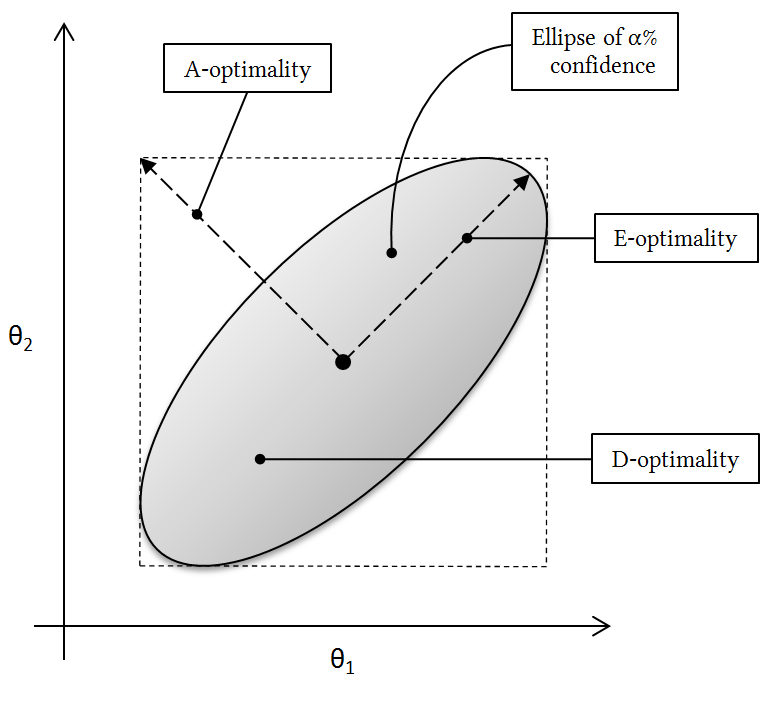
\epsfig{file=Figures/optimalcriterion.png, width=0.7\textwidth}\caption{Each criterion reduces the confidences intervals attempting to minimize one singular scalar value \cite{franceschini2008model}}
\label{fig:criteria}
\end{figure}

The question of which criteria to be used arises now. The D-optimal is the most used of the three standard criteria cited above. This is due to some exclusive appealing properties of the criterion \cite{franceschini2008model}:
\begin{itemize}
	\item Easy geometrical interpretation, as seen in Figure \ref{fig:criteria}.
	\item Invariance with respect to non-degenerated transformation applied to the model parameters, such as rescaling. This property is applied in equation (\ref{eq:Doptimality3}) in order to work, during the optimization process, with smaller quantities.
	\item Yielding to optimal experiments which correspond to replications of a small number of different experimental conditions.
	\item Optimal experiment design yields to non-singular FIM.
\end{itemize}
The main drawback this criterion has is that it gives too much importance to the parameter to which the model is most sensitive. Geometrically, this problem is equivalent to the idea of trying to minimize the volume of the ellipsoid by reducing mostly its bigger axis.

There are other criteria available for different purposes, like the modified E-optimality, that tries to maximize the FIM condition number, aiming to make the confidence ellipsoid as spherical as possible \cite{versyck1998optimal}. The correct application of this criterion would be in a case of strong parameter correlations, and the design will yield to a decoupled identification in parameters.

That is not the case in this thesis though. D-optimality will be the one used for the experiments designed for diabetic patients, and for every model tested.


